\documentclass[xcolor={dvipsnames}]{beamer}

\usetheme{Copenhagen}

\usecolortheme{whale}

\setbeamercolor*{palette tertiary}{use=structure,fg=white,bg=black}

\setbeamercolor*{palette quaternary}{fg=white,bg=black}

\setbeamercolor{frametitle}{bg=structure!75,fg=white}

\usepackage{amsmath}

\DeclareMathOperator{\trace}{trace}

\usepackage{graphicx}

\usepackage{fancybox}

\usepackage{array}

\usepackage{multirow}

\usepackage[numbers,square,sort]{natbib}

\usepackage[resetlabels]{multibib}

\usepackage{comment}

\usepackage{makeidx}

\usepackage{amsfonts}

\usepackage{amssymb}

\usepackage{blindtext}

\usepackage{multicol}

\usepackage{enumitem}

\usepackage[mathscr]{euscript}


\setlength{\columnsep}{1cm}

\makeatletter

\setbeamertemplate{headline}{}

\setbeamertemplate{footline}
{
	\leavevmode%

	\hbox{%
		
		\begin{beamercolorbox}[wd=.25\paperwidth,ht=2.25ex,dp=1ex,center]{author in 
		head/foot}%
			\usebeamerfont{author in head/foot}\insertshortauthor
		\end{beamercolorbox}%
		
		\begin{beamercolorbox}[wd=.55\paperwidth,ht=2.25ex,dp=1ex,center]{title in head/foot}%
			\usebeamerfont{title in head/foot}\insertshorttitle
		\end{beamercolorbox}%
		
		\begin{beamercolorbox}[wd=.2\paperwidth,ht=2.25ex,dp=1ex,right]{date in head/foot}%
			\usebeamerfont{date in head/foot}\insertshortdate{}\hspace*{2em}
			\insertframenumber{} / \inserttotalframenumber\hspace*{2ex} 
		\end{beamercolorbox}}%
	
	\vskip0pt%
}

\makeatother

\title {Las Vegas randomized algorithms in distributed consensus problems}

\author[Ghanei, Bateni, Rashidi]
{Narges Ghanei \and Aaron Bateni \and Fatemeh Rashidi  }    

\institute
{
	Department of Mathematics, Statistics and Computer Science,\\
	University of Tehran
}

\date[July 2022]
{July 2022}

\begin{document}
	
		\maketitle
% Begin Narges's part__________________________________________________________
	\begin{frame}{Introduction}
		In recent years, distributed consensus, agreement, and
		flocking problems have gained much attention in the systems
		and control community.\\
		The objective of this paper is to present the average
		consensus problems from the unifying viewpoint of proba-
		bilistic and Las Vegas algorithms.
		
	\end{frame}

	\begin{frame}{Average consensus problems}
		There is a set of N
		agents that possess numerical values and communicate their
		values with their neighbors in an iterative way. The goal is
		that all agents eventually reach a common value, which is
		the average of the initial values of all agents.
		
	\end{frame}

	\begin{frame}{Goal}
		In this paper, we aim at clarifying two
		points:\\
        \begin{block}{points}
            I) Introduce randomized algorithms appearing 
            in several variations of average consensus problems.\\
            II) Show the difference in
            the classes of algorithms appearing in consensus problems
            and those in the probabilistic approach in control.
        \end{block}
		
		
	\end{frame}

	\begin{frame}{PROBABILISTIC APPROACH TO UNCERTAIN SYSTEMS}
		We introduce a robustness analysis problem where
		various uncertainties can be represented. Given
		a system containing uncertain components, the objective
		of robustness analysis is to find whether certain control
		properties hold for all uncertainties.
		
	\end{frame}

	\begin{frame}{Formulating uncertain systems}
		We first assume that the uncertainty in the system is
		represented by a real/complex matrix $\Delta$ and further that
		$\Delta$ belongs to a bounded set $\mathscr{B}$. On the other hand, the
		system property is measured by the performance function
		$J : \mathscr{B} \rightarrow \mathbb{R}$. The function $J$ is assumed to be a measurable
		function.\\
        We want to check
        whether a certain performance level $\gamma$ is guaranteed for
        all possible uncertainties $\Delta \in \mathscr{B}$.
        \begin{alertblock}{}
            \begin{equation}
                \label{eqn:1}
                J(\Delta ) \leqslant \gamma \textrm{ for all } \Delta \in \mathscr{B}
            \end{equation}
        \end{alertblock}
        
    \end{frame}

	\begin{frame}{Formulating uncertain systems}
        We consider two specific performance criteria using
        $J(\Delta )$. The first is the worst-case performance defined by
        \begin{alertblock}{}
            \begin{equation} 	
                J_{max}:= \sup_{\Delta \in \mathscr{B} }J(\Delta ) 
            \end{equation}
            The other is the average-case performance 
            \begin{equation*} 	
                J_{ave}:= E_{\Delta}(J(\Delta )) 
            \end{equation*}
            where $E_{\Delta}(J(\Delta ))$ denotes the expected 
            value of the performance function with respect to the uncertainty set $\mathscr{B}$.
        \end{alertblock}
        
        
    \end{frame}

	\begin{frame}{MONTE CARLO RANDOMIZED ALGORITHMS}
        \begin{block}{Definition}
            A Monte Carlo randomized algorithm
            (MCRA) is a randomized algorithm that may produce a
            result that is incorrect, but the
            probability of such an incorrect result is bounded.
        \end{block}
        
        This algorithm involves the computation of the
        empirical maximum, which is defined by  
        \begin{alertblock}{}
            \begin{equation*} 	
                \hat{J}_{max}:= \max_{i=1, 2, ..., N}J(\Delta ^{(i)}) 
            \end{equation*}
        \end{alertblock}
        
    \end{frame}

	\begin{frame}{MONTE CARLO RANDOMIZED ALGORITHMS}
        An MCRA for a decision problem is said to have one-sided 
        error if it always provides a correct solution in one
        of the possible instances, but may provide a wrong solution
        for the other one.
        \begin{center}
			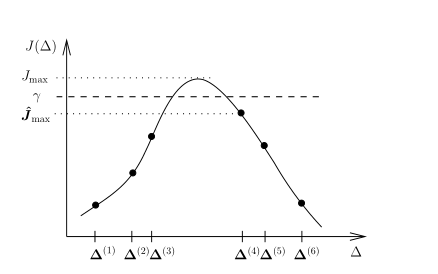
\includegraphics[width=0.49\linewidth]{1.png}
			One-sided MCRA: The worst-case performance when $\hat{J}_{max}<\gamma < J_{max}$
		\end{center}
        Two-sided error algorithms may produce
        a wrong solution for both instances when the answer is yes
        and no \cite{bib17}.
    \end{frame}

	\begin{frame}{LAS VEGAS RANDOMIZED ALGORITHMS}
        \begin{block}{Definition}
            Definition 2: Las Vegas randomized algorithms (LVRA)
            are randomized algorithms which always give the correct
            answer. The only difference from one run to another is the
            running time.
        \end{block}
        
    \end{frame}

% End Narges's part__________________________________________________________			
% Begin Aaron's part__________________________________________________________

	\begin{frame}{RQS}
        A well-known example is the \textit{Randomized Quick Sort (RQS)} \cite{bib14}, \cite{bib17}.
        \begin{examples}
            \textit{Example 1:} Given a set 
			
			\begin{equation*}
				\mathscr{S}_1 = {x_1 , . . . , x_N } 
			\end{equation*}
			
			of $N$ real numbers, consider the problem of sorting the numbers in an increasing order.
            The outline of the algorithm is as follows
			\begin{itemize}
				\item[1]
				Randomly select a number $x^{(1)}$ in the set $\mathscr{S}_1$.
				\item[2]
				Perform deterministic comparisons between $x^{(1)}$ and other elements in $\mathscr{S}_1$ .
                Let $\mathscr{S}^{(2)}$ be the set of numbers smaller than $x^{(1)}$ , 
                and let $\mathscr{S}^{(3)}$ be the set of numbers larger than $x^{(1)}$.
				\item[3]
				Recursively apply the two steps above to the sets $\mathscr{S}^{(2)}$ and $\mathscr{S}^{(3)}$. 
                Output the sorted version of $\mathscr{S}^{(2)}$, $x^{(1)}$, and then the sorted version 
                of $\mathscr{S}^{(3)}$.
			\end{itemize}
        \end{examples}
			
    \end{frame}

	\begin{frame}{RQS complexity}
        In a formal analysis, the running time is measured by the number of comparisons. 
        It follows that the expected running time is of order $O$($N$log$N$); 
        in fact, the running time is of this order with high probability, at least $1 − 1/N$ \cite{bib15}. 
        The \textbf{RQS} is more efficient than, for example, a deterministic brute-force approach, 
        which has complexity $O$($N^2$).
        
    \end{frame}

	\begin{frame}{LVRAs for uncertain decision problems}
        First, as the uncertainty set, we take a finite subset $\tilde{\mathscr{B}}$ of $\mathscr{B}$ with $N$ 
        elements given as
        \begin{equation*}
            \tilde{\mathscr{B}} = \left\{\tilde{\Delta}_1, \tilde{\Delta}_2, ..., \tilde{\Delta}_N\right\} 
            \subset \mathscr{B}
        \end{equation*}
        Assuming that the uncertain matrices in $\tilde{\mathscr{B}}$ are random variables,
        we consider a discrete probability measure; let the performance function 
        be $J : \tilde{\mathscr{B}} → \mathbb{R}$.
        The general robustness analysis problem is to find whether, for a given performance 
        level $\gamma > 0$, $J(\Delta) \leq \gamma$ for all $\Delta \in \tilde{\mathscr{B}}$. 
        The corresponding worst-case performance is
        \begin{alertblock}{}
            \begin{equation}
                J_{max} := \max_{\Delta \in \tilde{\mathscr{B}}}J(\Delta)
            \end{equation} 
        \end{alertblock}
        
    \end{frame}

	\begin{frame}{LVRA}
        The average case performance is
        \begin{alertblock}{}
            \begin{equation*}
                J_{ave} := E_\Delta\left[J(\Delta)\right] = \sum_{i=1}^N J(\tilde{\Delta}_i)Prob_\Delta(\tilde{\Delta}_i)
            \end{equation*}
        \end{alertblock}
        \begin{center}
            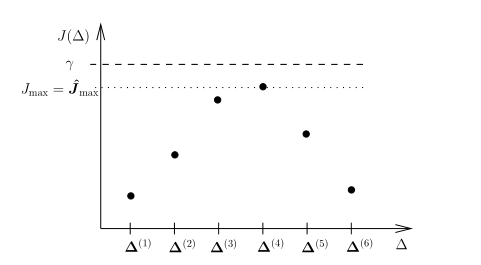
\includegraphics[width=0.49\linewidth]{2.png}
            LVRA: The worst-case performance when $J_{max} = \hat{J}_{max} < \gamma$
        \end{center}
    \end{frame}

    \begin{frame}{LAS VEGAS RANDOMIZED ALGORITHMS FOR DISTRIBUTED AVERAGE CONSENSUS}
		In this section, we present several problems in distributed average consensus where the application 
        of Las Vegas type algorithms can be effective and sometimes in fact crucial.
	\end{frame}
	
	\begin{frame}{General problem setup}
		Consider a network of $N$ nodes specified by the graph ($\mathscr{V}$, $\mathscr{E}$), 
        where $\mathscr{V} := {1, 2, . . . , N }$ is the set of nodes and $\mathscr{E}$ is the set of edges. 
        The graph is assumed to be undirected and connected. At time $k$, each node $i$ has a scalar value $x_i(k)$ 
        whose initial value is $x_i(0)$.
		
		\begin{block}{Goal}
			Provide an algorithm such that\\
			(i) the nodes update their values $x_i(k)$ using the information communicated from their neighbors.\\
			(ii) the values of the nodes eventually converge to the average of the initial values.
		\end{block}
	\end{frame}
	
	\begin{frame}{General problem setup}
		For a consensus algorithm, there are two elements that need to be determined: 
        The rules for the nodes to update their values and the neighbors with which each node should communicate.\\
		This problem is a particular version of distributed consensus.\\
		In the following, we consider three cases of this problem. The difference is in the 
        range of the node values:\\ \alert{Real numbers}, \alert{integer(quantized) numbers}, and \alert{binary numbers}. 
	\end{frame}
	
	\begin{frame}{Notation}
		Let the $N$-dimensional vector consisting of all node values at 
        time $k$ be $x(k) = [x_1(k) \hdots x_N(k)]^T$. The communication pattern 
        for the nodes at time $k$ is specified by the edge set $\tilde{\mathscr{E}}(k) \subset \mathscr{E}$, 
        i.e., if $\{i, j\} \in \tilde{\mathscr{E}}$, then $x_i(k)$ is updated using $x_j(k)$ and vice versa; 
        in this case, the nodes $i$ and $j$ are \emph{neighbors} of each other at this time. In general, 
        neighbors of a node may change over the time.
	\end{frame}
	
	\begin{frame}{Real-valued case}
			Average consensus is achieved when:
			\begin{equation}
				\lim_{k \rightarrow \inf} x_i(k) = \frac{1}{N} \sum_{j=1}^{N} x_j(0) \text{ for all } i = 1, ..., N.
			\end{equation}
		The update rule for the node $i$ takes a linear form as
		\begin{equation}
			x_i(k+1)=W_{ii}(k) x_i(k) + \sum_{j \in \mathscr{N}_i(k)} W_{ij}(k) x_j(k),
		\end{equation}
		\begin{equation}
			W_{ij}(k)=\begin{cases}
				\frac{1}{1+max\{d_{i}(k),d_{j}(k)\}} & \text{if }\{i,j\}\in \ensuremath{\tilde{\mathscr{E}}(k),}\\
				1-\sum_{l\in\mathscr{N}_{i}(k)}W_{il}(k) & \text{if }i=j\\
				0 & \text{otherwise,}
			\end{cases}
		\end{equation}
	\alert{$\mathscr{N}_i(k) := \{j : \{i, j\} \in \tilde{\mathscr{E}}(k)\}$}: The set of 
    neighbors for node $i$ at time $k$\\
	\alert{$W_{ij}(k)$}: Weights.\\
	\alert{$d_i(k)$: } The cardinality of $\mathscr{N}_i(k)$; neighbors for the node $i$.
	\end{frame}

	\begin{frame}{Real-valued case}
		The update rule in (5) can be implemented in a distributed and causal manner.\\
		Regarding the communication pattern specified by 
        $\tilde{\mathscr{E}}(k)$, $k \in \mathbb{Z}_+$, the assumption is as follows: 
        The graph ($\mathscr{V}$, $\bigcup_{s \geq k} \tilde{\mathscr{E}}(s)$) is a connected graph for all $k$.
		\begin{alertblock}{Notice}
			This theorem provides a condition on $\tilde{\mathscr{E}}(k)$ which must be 
            specified at the time of implementation for the average consensus in a deterministic sense.
		\end{alertblock}
	\end{frame}
	
	\begin{frame}{Real-valued case}
		A simple way to implement a communication pattern with the desired property is to employ 
        randomization: Each node $i$ communicates with a randomly and independently chosen neighbor 
        $j_k$ satisfying $\{i, j_k\} \in \mathscr{E}$ at time $k$. In particular, we allocate positive 
        probability to each edge $\{i, j\}$ in $\mathscr{E}$. Since ($\mathscr{V}$, $\mathscr{E}$) is a 
        connected graph, the condition on the communication pattern holds probabilistically. 
        Hence, the resulting algorithm achieves average consensus in (4) with probability one for any $x(0)$.	
	\end{frame}

% End Aaron's part__________________________________________________________			
% Begin Fateme's part__________________________________________________________

	\begin{frame}{Quantized-valued case}
		Here, by quantized, we mean that the node values are integers.\\
		To begin with, the average of the initial values may not be an integer.
		Thus, the target value is an integer approximation of the true average and is not
		necessarily unique. Moreover, consensus can be achieved in finite time because
		the nodes are updated in integers at each time instant.
	\end{frame}
	
	\begin{frame}{Quantized-valued case}
		the algorithm is said to achieve quantized average consensus if
		the following conditions hold:
		\begin{enumerate}[label=(\roman*)]
			\item The values are integers at all times: $x_{i}(k)\in \mathbb{Z}, \; \forall{i, k}$.
			\item The sum of the node values remains constant:
			$\sum_{i=1}^{N}x_{i}(k)=\sum_{i=1}^{N}x_{i}(0)$ for all $k$.
			\item All values converge to the quantized average: There exists $k^{*}$ such that 
			$x_{i}(k)\in \left\{ \overline{x}, \overline{x}+1 \right\}$ 
			for all $k > k^{*}$ 
			and $i$, where 
			$\overline{x}=\left\lfloor \sum_{i=1}^{N}x_{i}(0)/N \right\rfloor$.
		\end{enumerate}
	\end{frame}
	
	\begin{frame}{Quantized-valued case: quantized gossip algorithms}
		The following are the requirements for such algorithms: At time $k$, one edge 
		$\left\{ i, j \right\} \in \varepsilon$ 
		is selected at random in an i.i.d. fashion. Let 
		$D_{ij}(k)=\left| x_{i}(k)-x_{j}(k) \right|$.
		
		\begin{enumerate}[label=(\alph*)]
			\item If $D_{ij}(k)=0$, then the values of the nodes $i$ and $j$ remain the same for time $k+1$.
			\item If $D_{ij}(k)=1$, then the values are exchanged, or
			\textit{swapped}, by
			\begin{equation}
				x_{i}(k+1)=x_(j)(k) \text{ and } x_{j}(k+1)=x_{i}(k).
			\end{equation}
			\item Otherwise, the updates in the values satisfy
			\begin{equation*}
				x_{i}(k+1)+x_{j}(k+1)=x_{i}(k)+x_{j}(k),
			\end{equation*}
			\begin{equation*}
				D_{ij}(k+1)< D_{ij}(k).
			\end{equation*}
		\end{enumerate}
		
		\begin{block}{Notice:}
			Algorithms in this class are by definition randomized.
		\end{block}
	\end{frame}
	
	\begin{frame}{Binary-valued case}
		The third consensus problem we study is when the agents
		take binary values $x_{i}(k) \in \left\{ 0,1 \right\}$ for all $i, k$. In particular,
		the problem we discuss here is known as the \textit{Byzantine
			agreement} problem in the field of distributed computing,
		see e.g. \cite{bib17}. We will show that in this case even stronger
		results in favor of randomized schemes can be obtained.
	\end{frame}
	
	\begin{frame}{Quantized-valued case}%example
		
		
		\begin{exampleblock}{Example}
			Consider the graph below. Initially, the node is given the value $i$ for $i = 1, 2, 3$ and, thus, the average value is $2$. 
			Suppose that we employ a deterministic, periodic scheme for the edge selection with period 3 by following $\left\{ 1, 2 \right\}, \left\{ 1, 3 \right\}, \left\{ 3, 2 \right\}, \left\{ 1, 2 \right\}, \ldots$.\\
			Hence, the set of node values remains $1$, $2$, and $3$ and will never reach the consensus values. In contrast, by randomly choosing the edges, average consensus is possible in a matter of a few steps. This is an attractive communication scheme for its simplicity.
		\end{exampleblock}
		\begin{center}
			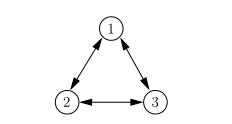
\includegraphics[width=0.3\linewidth]{3.png}
		\end{center}
	\end{frame}
	
	\begin{frame}{Binary consensus}
		We say that \textit{binary consensus} is
		achieved if each agent $i$ determines the \textit{decision value} $y_{i} \in \left\{ 0,1 \right\}$ such that
		\begin{enumerate}[label=(\roman*)]
			\item all nonfaulty agents arrive at the same decision value;
			
			\item if all nonfaulty agents have the same initial value
			$x_{i}(0)$, then they finish with $y_{i} = x_{i}(0)$.
		\end{enumerate}
	\end{frame}
	
	\begin{frame}{Algorithm}
		\begin{enumerate}[label=\arabic*)]
			\item At time $k$, send the value $x_{i}(k)$ to other agents and
			receive $x_{j}(k), \; j\neq i$, from them.
			
			\item Set the \textit{majority value} $m_{i}(k)\in \left\{ 0,1 \right\}$ to what the
			majority of agents sent as their values. Then, set the
			\textit{tally} $t_{i}(k)$ equal to the number of agents whose values
			are the same as $m_{i}(k)$.
			
			\item Now, depending on the result of the coin toss, let the
			\textit{threshold} $\overline{t}(k)$ be $L$ if the coin shows heads and $H$
			otherwise (note that the threshold is the same for all
			agents).
			
			\item Set the value $x_{i}(k)$ to the majority value $m_{i}(k)$ if
			$t_{i}(k) \ge \overline{t}(k)$ and to 0 otherwise.
			
			\item If the tally satisfies $t_{i}(k) \ge G$, then let the decision
			value $y_{i}$ be equal to $m_{i}(k)$.
		\end{enumerate}
	\end{frame}
	
	\begin{frame}{Binary-valued case}
		\begin{block}{Theorem 3}
			For the algorithm presented above, binary
			consensus is achieved with probability one for each initial
			condition $x(0) \in \left\{ 0,1 \right\}^{N}$. Moreover, the expected number of steps required is a constant.
		\end{block}
		
		\begin{alertblock}{Corollary}
			The consensus algorithm is an efficient Las Vegas type.
		\end{alertblock}
		
	\end{frame}
	
	\begin{frame}{CONCLUSION}
		In this paper, we discussed several variations of the
		average consensus problem and the role of probabilistic
		algorithms in this context. The class of Las Vegas randomized
		algorithms, which has been recently employed in the
		field of systems and control \cite{bib11}, \cite{bib24}, has been shown
		to be effective and sometimes crucial.
	\end{frame}
    \begin{thebibliography}{30}
	\begin{frame}{References}

        \bibitem{bib01} P. J. Antsaklis and J. Baillieul, Guest Editors. Special Issue on the Technology of Networked Control Systems.\textit{Proc. IEEE,} 95(1), 2007.
		
		
		\bibitem{bib02} J. Aspnes. Randomized protocols for asynchronous consensus. \textit{Distributed Computing}, 16:165–175, 2003.
		
		
		\bibitem{bib03} D. P. Bertsekas and J. N. Tsitsiklis.\textit{Parallel and Distributed Computation: Numerical Methods.} Prentice-Hall, Englewood Cliffs, NJ,1989.
		
		
		\bibitem{bib04} D. P. Bertsekas and J. N. Tsitsiklis. Comments on “Coordination of groups of mobile autonomous agents using nearest neighbor rules”. \textit{IEEE Trans. Autom. Control,} 52:968–969, 2007.
		
		
		\bibitem{bib05} V. D. Blondel, J. M. Hendrickx, A. Olshevsky, and J. N. Tsitsiklis. Convergence in multiagent coordination, consensus, and flocking. In \textit{Proc. 44th IEEE Conf. on Decision and Control and European Control Conf.,} pages 2996–3000, 2005.
		
		
		\bibitem{bib06} S. Boyd, A. Ghosh, B. Prabhakar, and D. Shah. Randomized gossip algorithms. \textit{IEEE Trans. Information Theory}, 52:2508–2530, 2006.

	\end{frame}

	\begin{frame}{References}

		\bibitem{bib07} R. Carli, F. Fagnani, M. Focoso, A. Speranzon, and S. Zampieri. Communication constraints in the average consensus problem. \textit{Automatica,} 44:671–684, 2008.
		
		
		\bibitem{bib08} M. Deng and Y.-C. Ho. An ordinal optimization approach to optimal control problems. \textit{ Automatica,} 35:331–338, 1999.
		
		
		\bibitem{bib09} M. J. Fisher, N. A. Lynch, and M. S. Paterson. Impossibility of distributed consensus with one faulty processor. \textit{J. ACM}, 32:374–382, 1985.
		
		
		\bibitem{bib10} Y. Hatano and M. Mesbahi. Agreement over random networks. \textit{IEEE Trans. Autom. Control,} 50:1867–72, 2005.
		
		
		\bibitem{bib11} H. Ishii and R. Tempo. Probabilistic sorting and stabilization of switched systems. Submitted for publication, 2007.
	 
        
        \bibitem{bib12} A. Jadbabaie, J. Lin, and A. S. Morse. Coordination of groups of mobile autonomous agents using nearest neighbor rules. \textit{IEEE Trans. Autom. Control}, 48:988–1001, 2003.
		
	\end{frame}

	\begin{frame}{References}
		
		\bibitem{bib13} A. Kashyap, T. Bas¸ar, and R. Srikant. Quantized consensus. \textit{Automatica}, 43:1192–1203, 2007.
		
		
		\bibitem{bib14} D. E. Knuth. \textit{The Art of Computer Programming,} 2nd edition, volume 3: Sorting and Searching. Addison-Wesley, Reading, MA, 1998.
		
		
		\bibitem{bib15} M. Mitzenmacher and E. Upfal. \textit{Probability and Computing: Randomized Algorithms and Probabilistic Analysis.} Cambridge University Press, 2005.
		
		
		\bibitem{bib16} L. Moreau.Stability of multiagent systems with time-dependent communication links.\textit{IEEE Trans. Autom. Control}, 50:169–182,2005.
		
		
		\bibitem{bib17} R. Motwani and P. Raghavan. \textit{Randomized Algorithms}. Cambridge University Press, 1995.
		
		
		\bibitem{bib18} R. Olfati-Saber and R. Murray. Consensus problems in networks of agents with switching topology and time-delays. \textit{IEEE Trans. Autom. Control,} 49:1520–1533, 2004.
		
	\end{frame}

	\begin{frame}{References}
		
		\bibitem{bib19} M. O. Rabin. Randomized Byzantin generals. In \textit{Proc. Annual Symp. on Foundations of Computer Science}, pages 403–409, 1983.
		
		
		\bibitem{bib20} A. V. Savkin. Coordinated collective motion of groups of autonomous robots: Analysis of Vicsek’s model. \textit{IEEE Trans. Autom. Control,}49:981–983, 2004.
		
		
		\bibitem{bib21} A. Tahbaz-Salehi and A. Jadbabaie. Necessary and sufficient conditions for consensus over random independent and identically distributed switching graphs. In \textit{Proc. 46th IEEE Conf. on Decision and Control,} pages 4209–4214, 2007.
		
		
		\bibitem{bib22} R. Tempo, E. W. Bai, and F. Dabbene. Probabilistic robustness analysis: Explicit bounds for the minimum number of samples. \textit{Systems and Control Letters}, 30:237–242, 1997.
		
		
		\bibitem{bib23}  R. Tempo, G. Calafiore, and F. Dabbene. \textit{Randomized Algorithms for Analysis and Control of Uncertain Systems.} Springer, London, 2005.
		
		
		\bibitem{bib24} R. Tempo and H. Ishii. Monte Carlo and Las Vegas randomized algorithms for systems and control: An introduction. European J. Control, 13:189–203, 2007.
		
	\end{frame}

	\begin{frame}{References}
	
		\bibitem{bib25} J. N. Tsitsiklis. \textit{Problems in Decentralized Decision Making and Computation}. PhD thesis, Dept. of Electrical Engineering and Computer Science, MIT, 1984. \href{http://web.mit.edu/jnt/www/Papers/PhD-84-jnt.pdf.}{http://web.mit.edu/jnt/www/Papers/PhD-84-jnt.pdf.}
		
		
		\bibitem{bib26} M. Vidyasagar. Statistical learning theory and randomized algorithms for control. \textit{IEEE Control Systems Magazine,} 18(6):69–85, 1998
		
		
		\bibitem{bib27} C. W. Wu. Synchronization and convergence of linear dynamics in random directed networks. \textit{IEEE Trans. Autom. Control,} 51:1207–1210, 2006.
		
		
		\bibitem{bib28} L. Xiao, S. Boyd, and S. Lall. A scheme for robust distributed sensor fusion based on average consensus. In \textit{Proc. Conf. on Information Processing in Sensor Networks,} pages 63–70, 2005.
			
	\end{frame}
\end{thebibliography}

\end{document}

	

